\documentclass[10pt]{article}
\usepackage[total={170mm,230mm}]{geometry}

\usepackage{cmap}
\usepackage{hyperref}
\usepackage[utf8]{inputenc}
\usepackage[T2A]{fontenc}
\usepackage[russian]{babel}

\usepackage{graphicx}
\usepackage{xcolor}
\usepackage{amssymb}
\usepackage{amsfonts}
\usepackage{amsmath}
\usepackage{amsthm}
\usepackage{physics}
\usepackage{wrapfig}
\usepackage{cancel}
\usepackage{pdfpages}
\usepackage{hyperref}
\usepackage{caption}
\usepackage{subcaption}
% \usepackage{bibtex}

\title{Домашнее задание №4. Метод подбора постоянной связи}
\author{Александр Козлов}
\date{\today}

\begin{document}

\maketitle

\section*{Формулировка задания}

Дан гамильтониан одномерной квантово-механической системы с потенциалом в виде гауссовой ямы
\begin{equation}
    H = - \dv[2]{}{x} + V_0\, e^{-x^2},
\end{equation}
где $V_0 < 0$. Требуется с помощью метода подгонки константы связи:
\begin{enumerate}
 \item найти основное состояние;
 \item[2*.] найти возбужденные состояния.
\end{enumerate}


\section{Дискретизация задачи}

Рассматриваемое уравнение Шрёдингера (УШ) имеет вид
\begin{equation}
    -\dv[2]{\psi}{x} + V_0\, e^{-x^2}\, \psi  = E\, \psi
    \label{eq:SE}
\end{equation}
или
\begin{equation}
    \dv[2]{\psi}{x}  + (E - V_0\, e^{-x^2})\, \psi  = 0.
\end{equation}
Стоит заметить, что такое уравнение соответствует обычному одномерному УШ при $\hbar=1$ и $m=1/2$.

Прежде всего зададим равномерную сетку
\begin{equation}
    x_0 = -R,\; x_1 = x_0 + \delta,\; x_2 = x_0 + 2\delta,\; \ldots,\; x_k = x_0 + k\delta,\; \ldots,\; x_M = x_0 + M \delta = R
\end{equation}
с шагом $\delta = 2R/M$, где $M$~---~целое положительное число, а $R$~---~положительное действительное число. Будем пользоваться численной аппроксимацией второй производной
\begin{equation}
    \dv[2]{\psi}{x}(x_k) = \dfrac{\psi(x_{k+1}) - 2\psi(x_{k}) + \psi(x_{k-1})}{\delta^2} + O(\delta^2),\quad k = \overline{1,M-1}
\end{equation}
и сводить уравнение \eqref{eq:SE} к задаче диагонализации трёхдиагональной матрицы.

Перед тем, как писать явный вид такой матрицы, необходимо поговорить о том, как будут задаваться граничные условия. Ясно, что волновые функции состояний дискретного спектра будут экспоненциально затухать при больших по абсолютному значению $x$. Это обстоятельство может быть численно учтено различными вариантами, однако, остановимся на варианте, при котором полагается $\psi(x_0) = \psi(x_M) = 0$. Тогда численное приближение УШ для $k=1$ примет вид
\begin{equation}
    -\dfrac{\psi(x_{2}) - 2\psi(x_{1})}{\delta^2} + V(x_1)\,\psi(x_1) = E\psi(x_1).
\end{equation}
Для $k=M-1$ получаем аналогичное уравнение
\begin{equation}
    -\dfrac{-2\psi(x_{M-1})+\psi(x_{M-2}) }{\delta^2} + V(x_{M-1})\,\psi(x_{M-1}) = E\psi(x_{M-1}).
\end{equation}
А для всех остальных $k$ имеем уравнение
\begin{equation}
    -\dfrac{\psi(x_{k+1}) - 2\psi(x_{k}) + \psi(x_{k-1})}{\delta^2} + V(x_k)\,\psi(x_k) = E\psi(x_k).
\end{equation}
В матричном виде задача записывается так:
\begin{equation}
\begin{split}
    &\begin{pmatrix}
        2\delta^{-2}+V(x_1)& -\delta^{-2}\\
        -\delta^{-2}& 2\delta^{-2}+V(x_2)& -\delta^{-2}\\
        % & -\delta^{-2}& 2\delta^{-2}+V_0\,e^{-x_3^2}& -\delta^{-2}\\
        & & & \ddots&\\
        & & & & -\delta^{-2}& 2\delta^{-2}+V(x_{M-2})& -\delta^{-2}\\
        & & & & & -\delta^{-2}& 2\delta^{-2}+V(x_{M-1})
    \end{pmatrix}
    \begin{pmatrix}
        \psi(x_1)\\
        \psi(x_2)\\
        \vdots\\
        \psi(x_{M-2})\\
        \psi(x_{M-1})
    \end{pmatrix}\\
    &=E
    \begin{pmatrix}
        \psi(x_1)\\
        \psi(x_2)\\
        \vdots\\
        \psi(x_{M-2})\\
        \psi(x_{M-1})
    \end{pmatrix}.
\end{split}
\end{equation}

\section{Применение операторной экспоненты}

Можно вместо нахождения собственных значений матрицы $\hat H$ перейти к нахождению собственных значе\-ний матрицы $\exp(\hat H T)$, где $T = \tau N$ --- значение мнимого времени, $N\gg1$, а $\tau<0$ --- достаточно малое значение мнимого времени ($\tau$ берётся отрицательным, чтобы наибольшим по модулю собственным значениям новой матрицы отвечали уровни энергии дискретного спетра гамильтониана). Применим к $\exp(\hat H \tau)$ формулу расщепления оператора
\begin{equation}
 \exp(\hat H \tau) = \exp((\hat T + \hat V) \tau) = \exp(\hat V \tau/2) \exp(\hat T \tau) \exp(\hat V \tau/2) + O(\tau^3).
\end{equation}
Матрица $\hat V$ является диагональной, экспонента от такой матрицы тоже будет диагональной. Для экспонен\-ты от матрицы кинетической энергии применим Паде-аппроксимацию
\begin{equation}
 \exp(\hat T \tau) = \qty(\hat I + \hat T \tau/2) \qty(\hat I - \hat T \tau/2)^{-1} + O(\tau^3).
\end{equation}
Таким образом удаётся аппроксимировать матрицу $\exp(\hat H T)$ матрицей $\hat A(\tau, N)$
\begin{equation}
 \exp(\hat H T) \approx \hat A(\tau, N) = \qty(\exp(\hat V \tau/2) \qty(\hat I + \hat T \tau/2) \qty(\hat I - \hat T \tau/2)^{-1} \exp(\hat V \tau/2) )^N.
\end{equation}
Таким образом, остаётся лишь найти собственные значения матрицы $\hat A(\tau, N)$, для чего следует использо\-вать итерации Арнольди.

\section{Реализация и результаты}

Рассмотрим случай $|V_0|=5.0$ и посмотрим как быстро считаются собственные значения гамильтониана предложенной схемой. На Рис. \ref{fig:T_vs_M_-5.0} показана зависимость времени работы алгоритма при различных значениях размера бокса.
\begin{figure}[htbp]
    \centering
    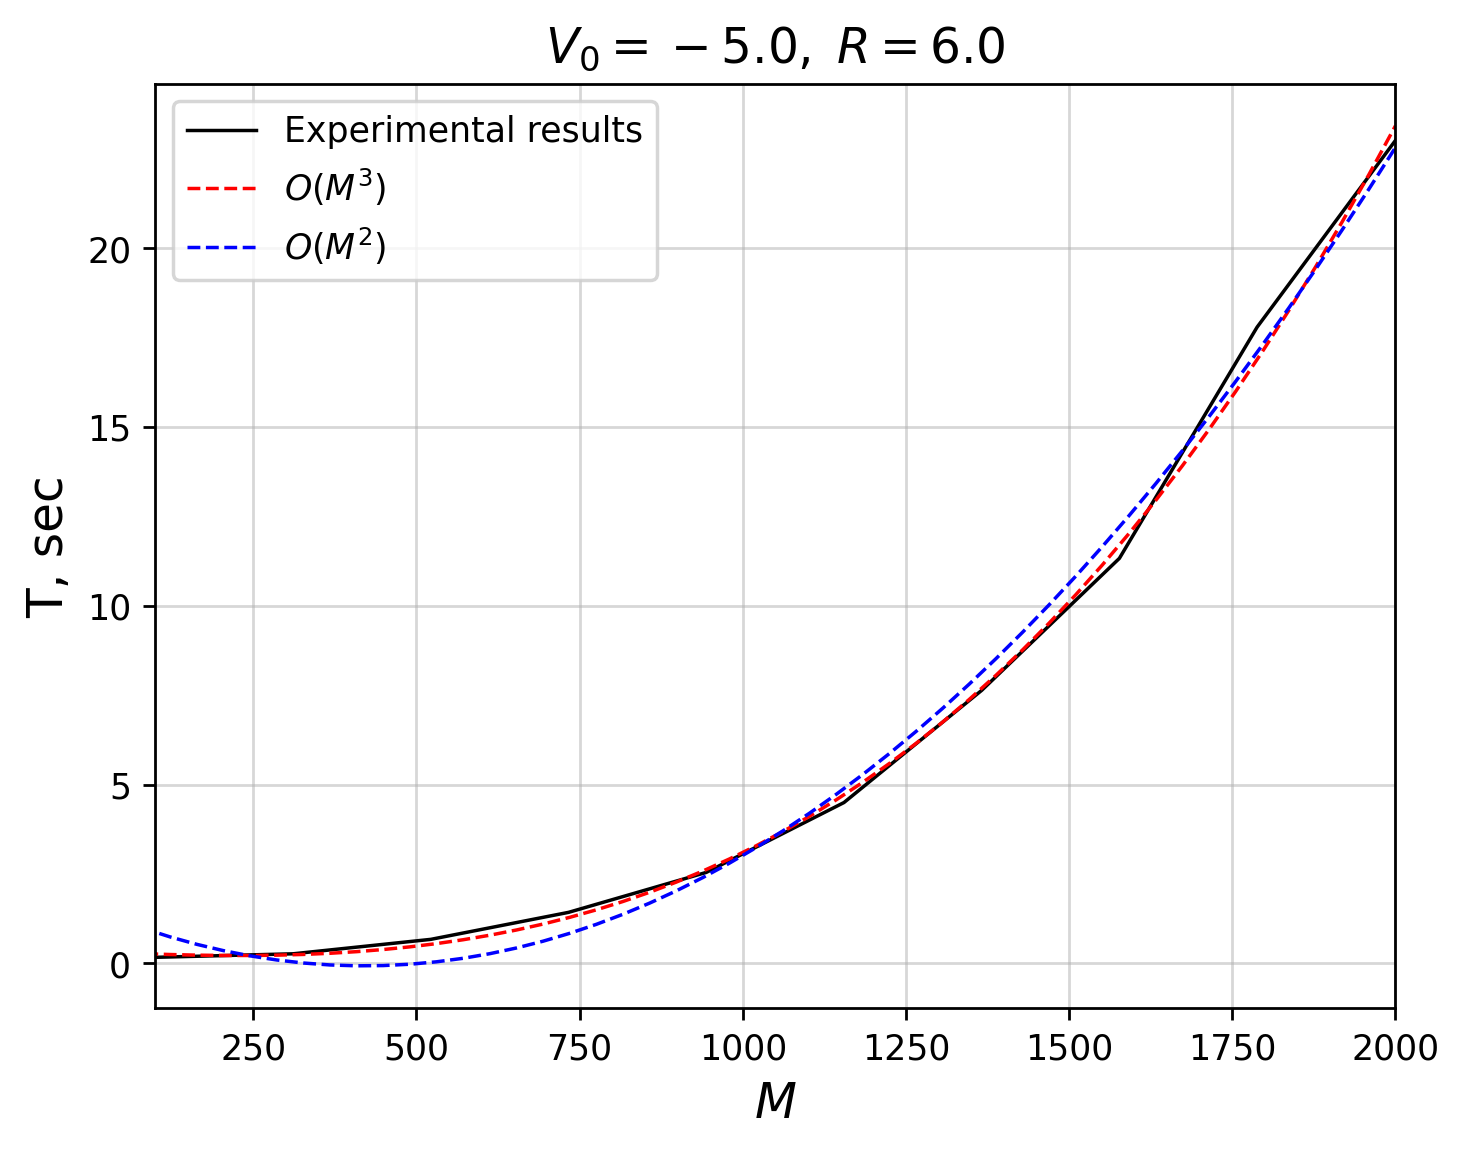
\includegraphics[width=0.75\textwidth]{../figures/T_vs_M_-5.0}
    \caption{Время работы алгоритма нахождения уровнений энергии дискретного спектра гамильтониана методом операторной экспоненты при различных размерах сетки $M$ в случае $R=6.0$ и $\abs{V_0}=5.0$, также приведены аппроксимации экспериментально полученной зависимости кубической и квадратичной параболами (красный и синий пунктир соответственно), откуда видно, что нельзя точно сказать кубическая или квадратичная зависимость времени вычисления от размера бокса.}
    \label{fig:T_vs_M_-5.0}
\end{figure}

Кроме того, было интересно посмотреть на зависимость невязки
\begin{equation}
 R = \abs{(\hat A - \lambda_i \hat I) \tilde \phi_i},
 \label{eq:residual}
\end{equation}
где $\lambda_i$ --- $i$-ое собственное значение оператора $\hat A$, а $ \tilde \phi_i$ --- соответствующая ему собственная функция, от параметра $\abs{\tau}$. Для этого кладём $N=10$, $M=1000$, $R=6.0$ и $\abs{V_0}=5.0$ и считаем невязку. Для основного состояния имеем зависимость, показанную на правой части Рис. \ref{fig:E_vs_tau_-5.0_e0}.
\begin{figure}[htbp]
    \centering
    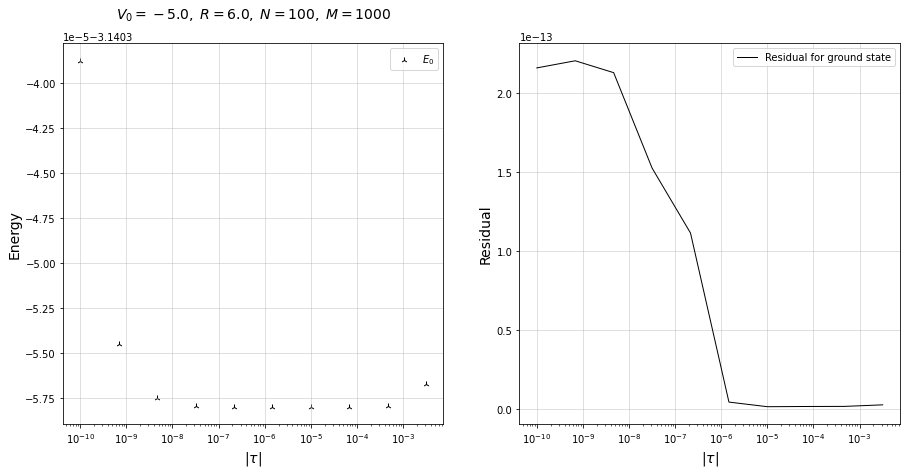
\includegraphics[width=\textwidth]{../figures/E_vs_tau_-5.0_e0}
    \caption{На левой панели показана зависимость вычисляемого уровня энергии основного состояния от $\abs{\tau}$ при  $N=10$, $M=1000$, $R=6.0$ и $\abs{V_0}=5.0$; на правой панели показана зависимость невязки \eqref{eq:residual} от $\abs{\tau}$ для основного состояния.}
    \label{fig:E_vs_tau_-5.0_e0}
\end{figure}
Для первого возбуждённого состояния имеем схожую картину (см. Рис. \ref{fig:E_vs_tau_-5.0_e1}).
\begin{figure}[htbp]
    \centering
    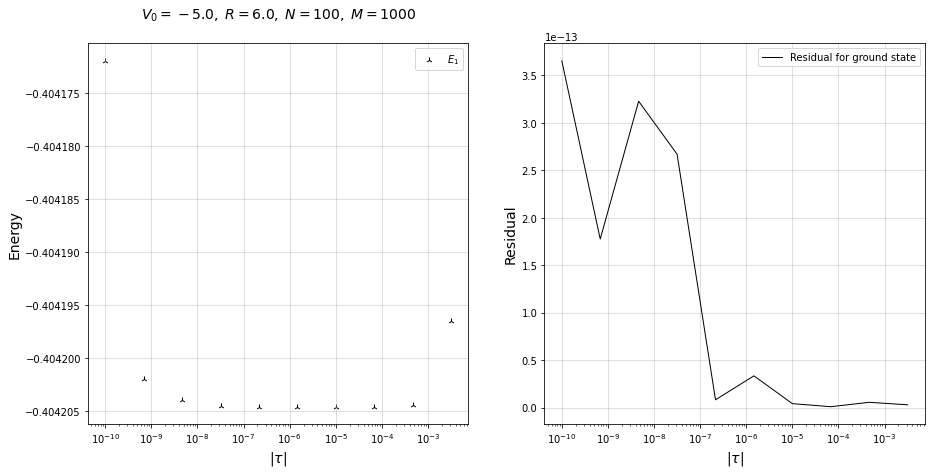
\includegraphics[width=\textwidth]{../figures/E_vs_tau_-5.0_e1}
    \caption{На левой панели показана зависимость вычисляемого уровня энергии первого возбуждённого состояния от $\abs{\tau}$ при  $N=10$, $M=1000$, $R=6.0$ и $\abs{V_0}=5.0$; на правой панели показана зависимость невязки \eqref{eq:residual} от $\abs{\tau}$ для первого возбужденного состояния.}
    \label{fig:E_vs_tau_-5.0_e1}
\end{figure}
\end{document}
